\documentclass{article} % For LaTeX2e
\usepackage{nips_adapted,times}
\usepackage{hyperref}
\usepackage{amsmath}
\usepackage{url}
\usepackage{listings}
\usepackage{xcolor}
\usepackage{graphicx}
\definecolor{codeblue}{rgb}{0.26, 0.44, 0.67}  % for keywords
\definecolor{codegreen}{rgb}{0.13, 0.54, 0.13} % for comments
\definecolor{codegray}{rgb}{0.5, 0.5, 0.5}     % for numbers
\definecolor{codeteal}{rgb}{0.16, 0.57, 0.57}  % for strings
\definecolor{backcolor}{rgb}{0.95, 0.95, 0.92} % background color

\lstdefinestyle{mypython}{
    backgroundcolor=\color{backcolor},   
    commentstyle=\color{codegreen}\itshape,
    keywordstyle=\color{codeblue}\bfseries,
    numberstyle=\tiny\color{codegray},
    stringstyle=\color{codeteal},
    basicstyle=\ttfamily\small,          % Main code font
    breakatwhitespace=false,             
    breaklines=true,                     
    captionpos=b,                        
    keepspaces=true,                     
    numbers=left,                        
    numbersep=5pt,                       
    showspaces=false,                    
    showstringspaces=false,
    showtabs=false,                      
    tabsize=4,
    frame=single,                        % Add a border around code block
    rulecolor=\color{codegray},
}

\lstset{style=mypython}  % Apply the style globally


\title{CS771: Mini-Project 2}


\author{
Chaitanya Vishwas Bramhapurikar \\
230305\\
\And
Om Ji Gupta\\
230719\\
\AND
Pranshu Agarwal \\
230776 \\
\And
Sunij Singh Gangwar \\
231051 \\
}

% The \author macro works with any number of authors. There are two commands
% used to separate the names and addresses of multiple authors: \And and \AND.
%
% Using \And between authors leaves it to \LaTeX{} to determine where to break
% the lines. Using \AND forces a linebreak at that point. So, if \LaTeX{}
% puts 3 of 4 authors names on the first line, and the last on the second
% line, try using \AND instead of \And before the third author name.

\newcommand{\fix}{\marginpar{FIX}}
\newcommand{\new}{\marginpar{NEW}}

\nipsfinalcopy

\begin{document}


\maketitle
\section{Task 1}
We started off with what was already given to us: LwP. We flattened the image and applied LwP. The accuracy we obtained from doing so is not worth mentioning. We first normalized the data using \textbf{ImageNet} statistics and then we tried different pre-trained feature extractors (\textbf{resnet}). We then finally settled on \textbf{EfficientNet B0} as that was giving us the best accuracy. To get a better understanding about the data we tried to visualize the data using \textbf{t-SNE}. 

\begin{figure}[h!]
    \centering
    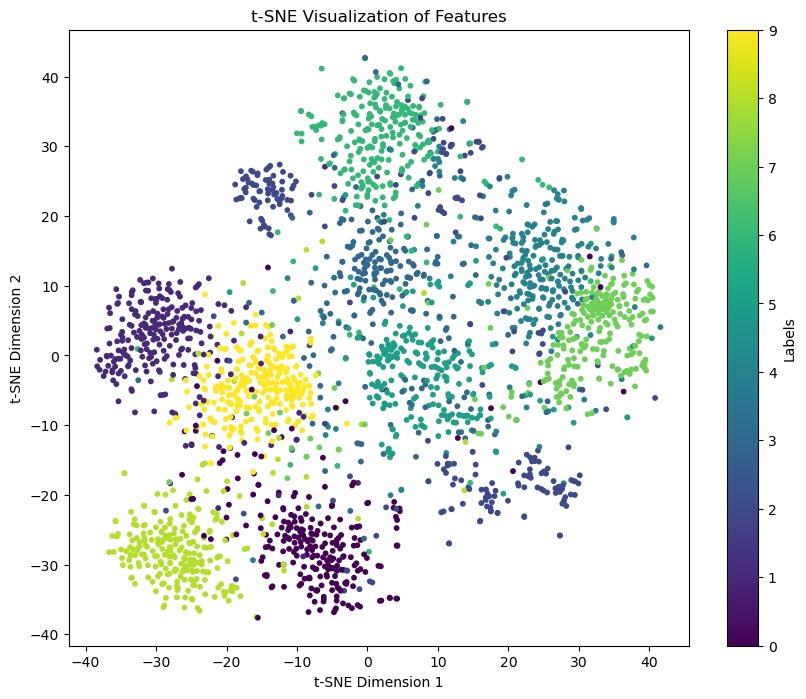
\includegraphics[width=0.7\linewidth]{mini-project-2/Plots/task1-tSNE.jpg}
    \caption{Data Visualization in Task 1}
    \label{fig:enter-label}
\end{figure}

We removed the classification layer of the feature extractor and then took features from its previous layer. We applied LwP on first labeled dataset yielding class prototypes for different classes. We applied our learned LwP on second dataset and learned pseudo labels. We then updated the current prototypes with a weighted average of current prototypes and pseudo labels data means. We gave more weightage to current prototypes. This acted as a regularization method. We got the following accuracy matrix:
\section*{Final Accuracy Matrix}

\[
\begin{array}{c|cccccccccc}
 & D_1 & D_2 & D_3 & D_4 & D_5 & D_6 & D_7 & D_8 & D_9 & D_{10} \\
\hline
f_1  & 0.8468 &       &       &       &       &       &       &       &       &       \\
f_2  & 0.8428 & 0.8472 &       &       &       &       &       &       &       &       \\
f_3  & 0.8444 & 0.8452 & 0.8344 &       &       &       &       &       &       &       \\
f_4  & 0.8396 & 0.8440 & 0.8340 & 0.8384 &       &       &       &       &       &       \\
f_5  & 0.8356 & 0.8400 & 0.8344 & 0.8388 & 0.8416 &       &       &       &       &       \\
f_6  & 0.8336 & 0.8356 & 0.8268 & 0.8336 & 0.8388 & 0.8308 &       &       &       &       \\
f_7  & 0.8324 & 0.8352 & 0.8228 & 0.8320 & 0.8376 & 0.8308 & 0.8192 &       &       &       \\
f_8  & 0.8300 & 0.8328 & 0.8188 & 0.8308 & 0.8356 & 0.8272 & 0.8140 & 0.8268 &       &       \\
f_9  & 0.8272 & 0.8316 & 0.8200 & 0.8292 & 0.8356 & 0.8268 & 0.8144 & 0.8252 & 0.8132 &       \\
f_{10} & 0.8276 & 0.8312 & 0.8204 & 0.8248 & 0.8360 & 0.8228 & 0.8156 & 0.8236 & 0.8100 & 0.8452 \\
\end{array}
\]

\section{Task 2}
We first tried same approach as Task 1 but we didn't get good enough accuracy. We later visualized the evaluation datasets D11, D12 using t-SNE. We get the following plot:

\begin{figure}[!h]
    \centering
    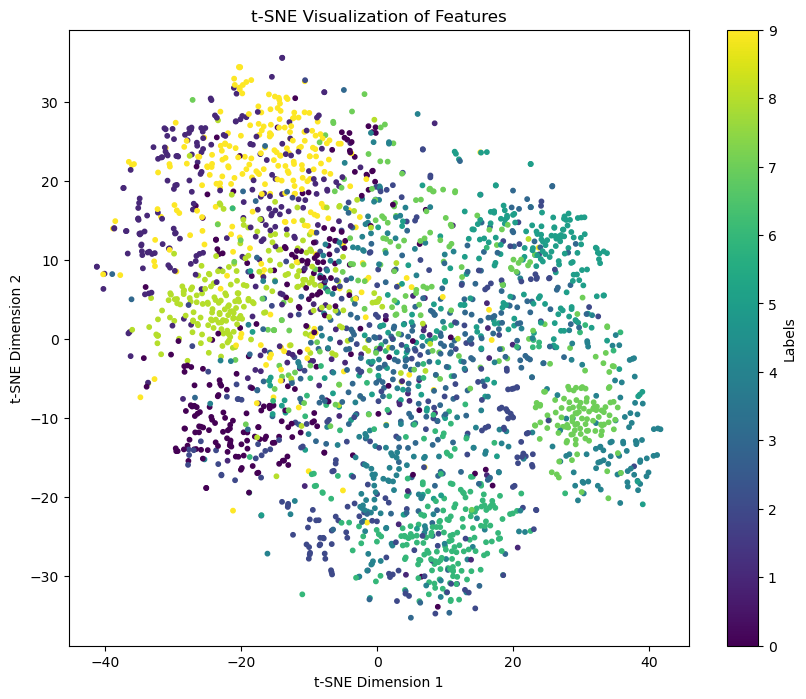
\includegraphics[width=0.7\linewidth]{mini-project-2/Plots/task2-tSNE.png}
    \caption{Data Visualization in Task 2}
    \label{fig:enter-label}
\end{figure}

We infer from the above plot that the classes overlap very much. So we went on to tried approaches that were discussed in the second research paper. We implemented \textbf{Prototype Contrastive Alignment} from the paper. We took into account the features with their assigned prototypes based on pseudo-labels and used cosine similarity between features and prototypes as logits, and applied cross-entropy loss to penalize misalignment. We also aligned the predictions of the current model with the previous model and used KL divergence to minimize the difference between the previous softmax probabilities and the current's. The expression for the CE-loss is: 

$$\mathcal{L}_{\text{CE}} = \mathbb{E}_{\textbf{x}_i \sim \mathcal{P}_X^t} \left[ - \sum_{k=1}^K \mathbb{I}_{\hat{y}_i = k} \log \frac{\exp \left( p_k^{t \top} f_\theta(\textbf{x}_i) + b_k \right)}{\sum_{c=1}^K \exp \left( p_c^{t \top} f_\theta(\textbf{x}_i) + b_c \right)} \right]$$
where $p_k^t$ are nothing but our prototype vectors for class $k$ at $t$-th domain. 

To account for the similarity of $f_\theta(\text{x}_i)$ (the extracted features of $\text{x}_i$) with the current $p_k^t$ as well as with the previous $p_k^{t - 1}$, loss corresponding to prototype contrastive alignment would be: 
\[\mathcal{L}_{PCA} = \mathbb{E}_{\textbf{x}_i \sim \mathcal{P}_X^t} \left\{\sum_{k=1}^K -\mathbb{I}_{\hat{y}_i = k} \log \frac{\exp \left( p_k^{t \top} f_\theta(\textbf{x}_i) \right) + \exp \left( p_k^{t-1 \top} f_\theta(\textbf{x}_i) \right)}{\Delta}\right \}
\]
where 
$$ \Delta = \sum_{c=1}^K \exp \left( p_c^{t \top} f_\theta(\textbf{x}_i) \right) + \sum_{c=1}^K \exp \left( p_c^{t-1 \top} f_\theta(\textbf{x}_i) \right) +\sum_{\textbf{x}_j \in T^t, j \neq i} \mathbb{I}_{\hat{\textbf{y}}_i \neq \hat{\textbf{y}}_j} \exp \left( f_\theta(\textbf{x}_i)^{\top} f_\theta(\textbf{x}_j) \right) $$

The expression for the KL-divergence is: 
$$\mathcal{L}_{\text{DIS}} = \mathcal{D}_{\text{KL}} [g_\omega^{t-1} (f_\theta^{t-1} (x)) \| g_\omega^t (f_\theta^t(\text{x}))]_{\text{x} \sim \mathcal{P}_X^{\mathcal{T}^t}}$$
which basically accounts for minimizing the current softmax probabilities with the previous ones. Combining all these losses at each domain, we get the following accuracy matrix: 
\section*{Final Accuracy Matrix}


\[
\resizebox{\textwidth}{!}{$
\begin{array}{c|cccccccccccccccccccc}
 & D_1 & D_2 & D_3 & D_4 & D_5 & D_6 & D_7 & D_8 & D_9 & D_{10} & D_{11} & D_{12} & D_{13} & D_{14} & D_{15} & D_{16} & D_{17} & D_{18} & D_{19} & D_{20} \\
\hline
f_1  & 0.8468 &       &       &       &       &       &       &       &       &       &       &       &       &       &       &       &       &       &       &       \\
f_2  & 0.8468 & 0.8476 &       &       &       &       &       &       &       &       &       &       &       &       &       &       &       &       &       &       \\
f_3  & 0.8468 & 0.8476 & 0.8404 &       &       &       &       &       &       &       &       &       &       &       &       &       &       &       &       &       \\
f_4  & 0.8468 & 0.8476 & 0.8404 & 0.8436 &       &       &       &       &       &       &       &       &       &       &       &       &       &       &       &       \\
f_5  & 0.8468 & 0.8476 & 0.8404 & 0.8436 & 0.8464 &       &       &       &       &       &       &       &       &       &       &       &       &       &       &       \\
f_6  & 0.8468 & 0.8476 & 0.8404 & 0.8436 & 0.8464 & 0.8412 &       &       &       &       &       &       &       &       &       &       &       &       &       &       \\
f_7  & 0.8468 & 0.8476 & 0.8404 & 0.8436 & 0.8460 & 0.8412 & 0.8368 &       &       &       &       &       &       &       &       &       &       &       &       &       \\
f_8  & 0.8468 & 0.8476 & 0.8404 & 0.8436 & 0.8464 & 0.8412 & 0.8368 & 0.8432 &       &       &       &       &       &       &       &       &       &       &       &       \\
f_9  & 0.8468 & 0.8476 & 0.8404 & 0.8436 & 0.8464 & 0.8412 & 0.8368 & 0.8432 & 0.8368 &       &       &       &       &       &       &       &       &       &       &       \\
f_{10} & 0.8468 & 0.8476 & 0.8404 & 0.8436 & 0.8464 & 0.8416 & 0.8368 & 0.8432 & 0.8368 & 0.8648 &       &       &       &       &       &       &       &       &       &       \\
f_{11} & 0.8468 & 0.8476 & 0.8404 & 0.8436 & 0.8464 & 0.8416 & 0.8368 & 0.8432 & 0.8368 & 0.8648 & 0.6940 &       &       &       &       &       &       &       &       &       \\
f_{12} & 0.8468 & 0.8476 & 0.8404 & 0.8436 & 0.8460 & 0.8416 & 0.8368 & 0.8432 & 0.8368 & 0.8648 & 0.6940 & 0.5384 &       &       &       &       &       &       &       &       \\
f_{13} & 0.8468 & 0.8476 & 0.8404 & 0.8436 & 0.8460 & 0.8416 & 0.8368 & 0.8432 & 0.8368 & 0.8648 & 0.6944 & 0.5384 & 0.7472 &       &       &       &       &       &       &       \\
f_{14} & 0.8468 & 0.8476 & 0.8404 & 0.8436 & 0.8460 & 0.8416 & 0.8368 & 0.8432 & 0.8368 & 0.8648 & 0.6944 & 0.5384 & 0.7472 & 0.7916 &       &       &       &       &       &       \\
f_{15} & 0.8468 & 0.8476 & 0.8408 & 0.8436 & 0.8460 & 0.8416 & 0.8368 & 0.8432 & 0.8368 & 0.8648 & 0.6944 & 0.5384 & 0.7472 & 0.7920 & 0.8300 &       &       &       &       &       \\
f_{16} & 0.8468 & 0.8476 & 0.8408 & 0.8436 & 0.8460 & 0.8416 & 0.8368 & 0.8432 & 0.8368 & 0.8648 & 0.6944 & 0.5384 & 0.7472 & 0.7920 & 0.8300 & 0.7128 &       &       &       &       \\
f_{17} & 0.8468 & 0.8476 & 0.8408 & 0.8436 & 0.8460 & 0.8416 & 0.8372 & 0.8428 & 0.8368 & 0.8648 & 0.6940 & 0.5384 & 0.7472 & 0.7920 & 0.8300 & 0.7128 & 0.7228 &       &       &       \\
f_{18} & 0.8468 & 0.8476 & 0.8404 & 0.8436 & 0.8460 & 0.8416 & 0.8372 & 0.8432 & 0.8368 & 0.8648 & 0.6944 & 0.5384 & 0.7472 & 0.7916 & 0.8300 & 0.7124 & 0.7228 & 0.7252 &       &       \\
f_{19} & 0.8468 & 0.8476 & 0.8404 & 0.8436 & 0.8460 & 0.8416 & 0.8372 & 0.8432 & 0.8368 & 0.8648 & 0.6944 & 0.5384 & 0.7472 & 0.7916 & 0.8300 & 0.7124 & 0.7228 & 0.7256 & 0.6300 &       \\
f_{20} & 0.8468 & 0.8476 & 0.8404 & 0.8436 & 0.8460 & 0.8416 & 0.8372 & 0.8432 & 0.8368 & 0.8648 & 0.6944 & 0.5380 & 0.7472 & 0.7916 & 0.8300 & 0.7124 & 0.7228 & 0.7256 & 0.6300 & 0.8104 \\
\end{array}
$}
\]

This can be considered as our final improved approach for task 1 as well. 

\section{Relevant Links/Acknowledgements}
\begin{itemize}
    \item We took help of chat-gpt/claude in debugging. 
    \item The presentation slides corresponding to problem 2 can be found at \href{https://drive.google.com/file/d/16M1vzTdMby0obWokpMC8oeYKSnHBBGg9/view?usp=drive_link}{this} link. 
    \item The corresponding research paper can be found at \href{https://arxiv.org/pdf/2301.10418}{this} link. 
    \item The youtube link for the explanation video can be found \href{https://youtu.be/y78fq7vCHi4?si=6zj9N_54JkJj3Ery}{here}.
\end{itemize}

\end{document}
